% Copyright (c) 2017-2019 Michael C. Heiber
% This file is part of the Excimontec project, which is subject to the MIT License.
% For more information, see the LICENSE file that accompanies this software.
% The Excimontec project can be found on Github at https://github.com/MikeHeiber/Excimontec

\documentclass[%
 reprint,onecolumn,notitlepage,
superscriptaddress,longbibliography,
 amsmath,amssymb,
 aps,rmp,floatfix,
]{revtex4-1}
\bibliographystyle{unsrtnat}
\setcitestyle{numbers,square}

\usepackage[margin=1in]{geometry}
\usepackage[utf8]{inputenc}
\usepackage{amsmath}
\usepackage{hyperref}
\usepackage{minted}
\usepackage[version=4]{mhchem}

\begin{document}

\title{Excimontec v1.0 User Manual}
\author{Michael C. Heiber}

\date{\today}

\maketitle

\tableofcontents

\section{Introduction}

Kinetic Monte Carlo simulations are a powerful computational tool that have been used in concert with experiments and more detailed theoretical methods to understand and optimize organic semiconductor materials and devices.\cite{heiber2019chapter} 
However, despite over 30 years of applying KMC tools to organic semiconductors, no widespread or standardized software tools have taken hold in the community. 
Instead, many research groups around the world have maintained private codebases of varying complexity, efficiency, and reliability. 
As a result, there have been large barriers to entry for new researchers and a lot of repeated effort throughout the community that would be much better off applied to pushing the capabilities of the technique and further refining the physical models.

Excimontec represents an honest effort to bring the community together around a well-tested, optimized, reliable, and accessible open-source tool for performing KMC simulations of organic electronic devices. 
The current version (v1.0) implements a cubic lattice-based model for the organic semiconductor layer and is focused on simulation tests for neat single carrier diodes and binary donor-acceptor organic photovoltaic devices.
Future extension of the software to simulate light emitting diodes and transistors is planned.
The software is written in modern C++ and is optimized for efficient pleasingly parallel execution on high performance computing clusters using MPI. 
This software package uses object-oriented design and extends the KMC\_Lattice framework.\cite{heiber2019joss1} 

\section{Simulation Tests}

Excimontec is designed to allow users to select and run a particular simulation test with a specific set of input parameters.
Currently there are five different simulations tests available:
\begin{enumerate}
    \item Exciton Diffusion Test
    \item Time-of-Flight Charge Transport Test
    \item Internal Quantum Efficiency Test
    \item Dynamics Test
    \item Steady State Charge Transport Test
\end{enumerate}
These choices are made within the parameter file that is then passed as an input argument to the program.
An example parameter file (parameters\_default.txt) is provided in root repository directory to be used as a starting point.
A valid parameter file has strict formatting rules, so users should simply copy the default parameter file and then modify the values as needed.
The program should generate an error message if you accidentally mess up the formatting or put an invalid value for any of the parameters.
Below, the basics of each simulation test is explained and some examples of the types of physical behavior that can be simulated are provided.
If you have further questions about the capabilities and options for any of the simulation tests, please post an Issue on the Github website.

\subsection{Exciton Diffusion Test}

This simulation mode is designed to allow users to test exciton diffusion behavior under a variety of different conditions.
The simulation is performed by randomly placing excitons one at a time on the lattice, letting them diffuse via their normal hopping mechanism, and finally recording the displacement distance upon exciton recombination.
The simulation is performed independently on each processor core until the number of tested excitons reaches the specified N\_tests value from the parameter file.
The independent results from each processor are then aggregated and the mean and standard deviation of the diffusion length are calculated.

When performed on a neat material, one can determine how properties like energetic disorder, temperature, exciton hopping rate, and exciton lifetime affect the diffusion length.
For example, Fig. \ref{fig:exciton_diffusion_example}(a) shows how the exciton diffusion length increases as the singlet exciton hopping rate prefactor increases in a neat material with an uncorrelated Gaussian density of states.
Then, Fig. \ref{fig:exciton_diffusion_example}(b) shows how the exciton diffusion length decreases as the energetic disorder increases and slows down the diffusion process.
These types of simulations are a good way to determine the materials parameters required to reach a desired exciton diffusion length or to probe 

\begin{figure}[h]
    \centering
    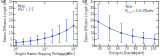
\includegraphics{Exciton_diffusion_example_data.pdf}
    \caption{Exciton diffusion test data showing how the exciton diffusion length depends on (a) the exciton hopping rate prefactor and (b) the energetic disorder of the material.}
    \label{fig:exciton_diffusion_example}
\end{figure}

\subsection{Time-of-Flight Charge Transport Test}

This simulation mode is designed to reproduce an ideal time-of-flight (ToF) charge transport experiment.
In the ToF experiment, a very thin sheet of charge carriers is generated at one surface of film by a laser pulse and then the transient current response is measured as the charge carriers move through the film and are eventually extracted at the opposite electrode.
ToF experiments have been widely used to probe the fundamental charge transport behavior of organic semiconductors as a function of electric field, temperature, charge carrier density, etc.
Whereas the experiment is limited in that information can only be extracted from analysis of the current transient, KMC simulations of the same test can provide additional information.
The ToF simulation mode in Excimontec simulates the transport of an ultrathin sheet of charge carriers (electrons or holes) through the lattice and provides current density transients as well as the charge carrier density transient, average charge carrier occupation energy transient, average mobility transient, and transit time probability histograms.
Examples of these results are provided in Fig. \ref{fig:tof_example}(a) for a neat material.

\begin{figure}[h] % 16.5 cm column width
    \centering
    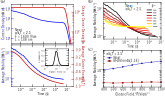
\includegraphics{ToF_example_data.pdf}
    \caption{Time-of-flight charge transport test results showing (a) neat material transients, (b) neat material electric-field-dependent mobility relaxation, and (c) electric-field-dependent steady-state mobility in a neat material and a bulk heterojunction blend.}
    \label{fig:tof_example}
\end{figure}

This provides users with a detailed tool to probe the transient mobility relaxation phenomena and how it is affected by the density of states, temperature, electric field, charge carrier density, material morphology, etc. 
For example, Fig. \ref{fig:tof_example}(b) shows the how the transition from dispersive to nondispersive transport shifts with electric field in a neat material and how the steady state mobility increases as the electric field increases. 
The electric-field dependence of mobility can also be quantified in bulk heterojunction blends to determine the complex interplay between energetic disorder ($\sigma$) and domain network tortuosity ($\tau$) shown previously.\cite{heiber2017prapp2}

As more advanced features, users can also create the initial charge carriers at a specific energy position within the density of states instead of randomly populating it to probe how the starting energy of the charge carriers affects the transient behavior.
In addition, one can produce charge extraction maps to probe for fluctuations in current density across the area of the film that may arise due to energetic fluctuations from the correlated disorder model or morphological features in a bulk heterojunction film.

\subsection{Internal Quantum Efficiency Test}

The internal quantum efficiency (IQE) test allows users to simulate a common photovoltaic device characterization technique.
It is a steady state measurement that quantifies the fraction of absorbed photons that are successfully converted into extracted charge carriers. 
The measurement is commonly done under short-circuit conditions, but one can also apply a bias.
The IQE test additionally provides a detailed breakdown of the various loss mechanisms that produce the final IQE value, including the exciton dissociation yield, the charge separation yield, and the bimolecular recombination loss fraction.


\begin{figure}[h]
    \centering
    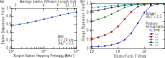
\includegraphics{IQE_example_data.pdf}
    \caption{Internal quantum efficiency test results showing (a) exciton dissociation yield in a BHJ morphology and (b) charge separation yield in a bilayer device architecture.}
    \label{fig:IQE_example}
\end{figure}

\subsection{Dynamics Test}

\begin{figure}[h]
    \centering
    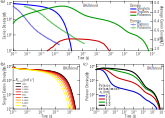
\includegraphics{Dynamics_example_data.pdf}
    \caption{Dynamics test results showing (a) full carrier density and energy transients, (b) exciton dissociation dynamics, and (c) polaron recombination dynamics in a BHJ blend.}
    \label{fig:dynamics_example}
\end{figure}

\subsection{Steady State Charge Transport Test}

\section{Simulation Parameters and Model Details}

Specifying which simulation test to run, which device architecture to simulate on, which mechanism models to use, and all of the electronic materials properties and parameters is done using the parameter file.
A single parameter file is used to run the KMC simulation test for a single set of parameters.
To do parameter sweeps, one must create separate parameter files for each condition and then run separate simulations for each.
While this can be tedious when manually creating and modifying the parameter files, bash scripts can be used to quickly create a series of parameter files for a parameter sweep and simulation job arrays can be used to submit all of the simulations in a parameter sweep and keep the individual simulations together.
This part with go through section of the parameter file and explain what each parameter is used for.

\subsection{KMC Algorithm Parameters}\label{sub:KMC_algorithms}

At any given time, there are a number of different mechanisms that can occur in an organic semiconductor device under operational conditions. 
Excitons and polarons can move, dissociate, recombine, etc. 
In a KMC simulation, each time the state of the system changes in any way, we say that an event has occurred. The goal of a KMC simulation is to simulate the evolution of the system over time, one event at a time, to determine the transient behavior or to gather statistics about the steady state behavior.

\subsubsection{First-reaction Method:}

Here, the formalism of the Gillespie first reaction method (FRM) is implemented to determine which event will occur next.\cite{gillespie1976jcp} 
In a system containing numerous excitons and polarons, there are number of different possible events that can occur at any given time. 
To determine when each will occur, the wait time for each possible event is calculated,
$$t = \frac{-\ln{X}}{R},$$
where $X$ is a random number between 0 and 1 chosen from a uniform distribution and $R$ is the rate of the particular event. 
With the wait time calculated for all possible events, the event with the shortest wait time is executed. 
An extension of this method is the assumption that the majority of excitons and polarons are independent and that the calculated events can be put into a sorted schedule queue to be executed one by one as their scheduled time comes. 
After each iteration, only a small number of newly disabled events must be removed from the queue and only a small number of newly enabled events must be calculated and added to the queue. 
As a result, all possible events do not need to be recalculated after each iteration.

\subsubsection{BKL Algorithm:}

One also does not need to store all possible events for each exciton or polaron since only one of them will be executed before calculating the next event for that exciton or polaron. 
To efficiently determine the chosen event among many possibilities for a single exciton or polaron, the Bortz-Kalos-Lebowitz algorithm is used.\cite{bortz1974prb}
Instead of drawing a random number to calculate the wait time for each possible mechanism, the event can be chosen with only a single random number. 
One first calculates the rates for all possible ($N$) events, places them in an array, and adds them up,
$$R_\text{sum} = \sum_{i=0}^N R_i$$
One then generates a single random number and then finds the smallest event index ($i=n$) such that,
$$\sum_{i=0}^n R_i > R_\text{sum}X.$$
The $n^\text{th}$ event becomes the selected event, and the wait time for the event is calculated using $R_\text{sum}$. 
With the BKL algorithm, the event queue remains relatively small since only one event is queued per exciton or polaron in the simulation.

\subsubsection{Event Recalculation}

However, polarons specifically have long-range electrostatic interactions with each other, and their events are not truly completely independent.
The motion of one or several polarons can modify the electrostatic potential landscape, which should have an impact on the next event of other nearby polarons. 
When using the first-reaction method, this impact is ignored to save computing time. 
If one wants to check the significance of this simplifying assumption, the full recalculation algorithm is also implemented and can be enabled in the parameter file. 
With the full recalculation method, all events for all excitons and polarons are recalculated after each iteration of the simulation, thereby ensuring that the next event takes into full consideration all changes to the system.

As an alternative, a selective recalculation method is also implemented that allows users to selectively update the events of all objects near the previous event within a user defined cutoff radius.\cite{heiber2012jcp} 
By choosing the optimal recalculation cutoff radius in the parameter file, users can ensure that there is minimal impact from the simplifying assumptions of the first-reaction method, while also saving considerable computational time relative to the full recalculation method.

\subsection{Lattice Parameters}

\subsection{Device Architecture Parameters}

Neat material
Donor-acceptor bilayer
Random donor-acceptor blend
bulk heterojunction morphology from Ising\_OPV

\subsection{Exciton Parameters and Mechanisms}

\subsubsection{Exciton Generation}

To simulate the creation of optically generated excitons, singlet excitons are created randomly on donor or acceptor sites based on the generation rates specified in the parameter file. 
Currently, the exciton generation model does not include any interference effects that can cause generation rate gradients in real devices. 
For calculating the singlet exciton generation rate,
$$R_\text{sxg} = G V.$$
where, $G$ is the exciton generation rate of the material and $V$ is the total volume of the material in the lattice.
It is assumed that no triplet excitons are generated by illumination due to the fact that it is a spin forbidden transition,
$$R_\text{txg} = 0.$$

\subsubsection{Exciton Hopping}

Transport of excitons from site to site can occur by two different mechanisms, F{\"o}rster resonance energy transfer (FRET)\cite{forster1948} or Dexter electron exchange.\cite{dexter1953jcp} 
Under different conditions, one of the two mechanisms usually dominates, so both mechanisms do not need to be calculated for every iteration of the simulation. 
Singlet excitons are generated optically and can also readily emit a photon. 
Due to this property, singlet excitons can move from site to site by emitting and then absorbing a virtual photon, and this longer-range process typically dominates over the Dexter electron exchange mechanism. 
Conversely, triplet excitons have spin forbidden optical transitions, thereby making photon emission and absorption very slow processes. 
As a result, the energy transfer mechanism is negligible and the shorter-range Dexter electron exchange mechanism dominates. 
With Dexter electron exchange, electrons on neighboring sites are exchanged via a charge transfer mechanism. 
The excited electron moves to a neighboring site, and the exciton effectively moves.

Regardless of the mechanism, the driving force of the transition is based on the initial and final state energies.
For singlet excitons, the state energy is defined
$$E_{\text{s}} = E_\text{HOMO} - E_\text{LUMO} - E_\text{B}$$
where $E_\text{HOMO}$ is the highest occupied orbital energy, $E_\text{LUMO}$ is the lowest unoccupied orbital energy, and $E_\text{B}$ is the exciton binding energy.
For triplet excitons, 
$$E_{\text{t}} = E_\text{s} - \Delta E_\text{ST}$$
where $\Delta E_\text{ST}$ is the singlet-triplet splitting energy.

\subsubsection*{\textbf{F{\"o}rster resonance energy transfer (FRET) model:}}

The rate for FRET-based singlet exciton hopping is defined
$$R_{\text{sxh,FRET},ij} = R_{0,\text{sxh}} \left( \frac{1}{d_{ij}} \right)^6 f_\text{B} \left( \Delta E_{\text{FRET},ij}\right),$$
where $R_{0,\text{sxh}}$ is the singlet exciton hopping prefactor, $d_{ij}$ is the distance between sites, and
$$\Delta E_{\text{FRET},ij} = E_{\text{s},j} - E_{\text{s},i}.$$
$f_\text{B}$ is the Boltzmann function,
$$f_\text{B} \left( \Delta E_{ij}\right) = \begin{cases}
\exp{\left( \frac{-\Delta E_{ij}}{k_\text{B} T} \right)} & \Delta E_{ij} > 0 \\
1 & \Delta E_{ij} \le 0 \\
\end{cases}$$
where $k_\text{B}$ is the Boltzmann constant and $T$ is the temperature.

\subsubsection*{\textbf{Dexter electron exchange model:}}

The rate for Dexter-based exciton hopping is defined
$$R_{\text{txh,Dex},ij} = R_{0,\text{txh}} \exp{\left(- 2 \gamma_{\text{t}} d_{ij} \right)} f_\text{B} \left( \Delta E_{\text{Dex},ij}\right),$$
where $R_{0,\text{txh}}$ is the triplet exciton hopping prefactor, $\gamma_{\text{t}}$ is the triplet localization parameter, and
$$\Delta E_{\text{Dex},ij} = E_{\text{t},j} - E_{\text{t},i}.$$

\subsubsection{Exciton Dissociation}

Exciton dissociation is essentially a transition from an exciton state to a charge-transfer (CT) state that spans a donor-acceptor interface. 
The event proceeds by a charge transfer mechanism. 
For an exciton located on a donor site, an electron transfers from the donor site to an acceptor site. 
For an exciton located on an acceptor site, a hole transfers from the acceptor site to a donor site. 
As a result, the mechanism is simulated using a charge transfer model. 
Excimontec implements two options for charge transfer models, the Miller-Abrahams phonon-assisted tunneling model\cite{miller1960pr} and a simplified Marcus model \cite{marcus1956jcp} that implements a polaronic mechanism.

Regardless of the model used, the driving force for this transition depends on the energies of the initial final states. For singlet excitons,
$$\Delta E_{\text{sxd},ij} = E_{\text{CT},ij} - E_{\text{s},i},$$
and for triplet excitons,
$$\Delta E_{\text{txd},ij} = E_{\text{CT},ij} - E_{\text{t},i},$$
where $E_{\text{CT},ij}$ is the CT state energy. 
For the dissociation of an exciton starting from a donor site, 
$$E_{\text{CT},ij} = E_{\text{HOMO}_\text{D},i} - E_{\text{LUMO}_\text{A},j} + E_\text{B,CT} \left( d_{ij} \right) + E_\text{C}(q_i) + E_\text{C}(q_j) - e \mathbf{d}_{ij} \cdot \mathbf{F},$$
where $E_\text{B,CT}$ is the CT state binding energy, $E_\text{C}(q)$ is the electrostatic interaction energy term for the newly formed polarons interacting with any other polarons in the system, $e$ is the elementary charge constant, $\mathbf{d}_{ij}$ is the CT state dipole displacement vector, and $\mathbf{F}$ is the internal electric field vector.
An analogous expression is used for dissociation of an an acceptor exciton.
The CT state binding energy is defined
$$E_\text{B,CT} \left( d_{ij} \right) = \frac{-e^2}{4 \pi \epsilon \epsilon_0 d_{ij}},$$
where $\epsilon$ is the dielectric constant and $\epsilon_0$ is the vacuum permittivity constant.
The electrostatic interaction energy between polarons is calculated via the summation
$$E_\text{C}(q_k) = \sum_{l,l\neq k} \frac{q_k q_l}{4 \pi \epsilon \epsilon_0 d_{kl}}, \quad d_{kl} \leq r_\text{C,cut},$$
which adds together the interaction energy between the new polaron on site $k$ having charge $q_k$ with all other polarons in the lattice where the distance between the two polarons on site $k$ and site $l$ ($d_{kl}$) is less than the Coulomb cutoff radius ($r_\text{C,cut}$).

However, users can also enable the Gaussian polaron delocalization model\cite{gagorik2015afm} to reduce the CT state binding energy. 
With this model enabled,
$$E_\text{B,CT,d} \left( d_{ij} \right) = \frac{-e^2}{4 \pi \epsilon \epsilon_0 d_{ij}} \text{erf}\left(\frac{d_{ij}}{\sigma_\text{p}\sqrt{2}}\right)$$
where $\sigma_\text{p}$ is the polaron delocalization length.
The Gaussian polaron delocalization model also modifies the polaron electrostatic interaction energy function, so that
$$E_\text{C,d}(q_k) = \sum_{l,l\neq k} \frac{q_k q_l}{4 \pi \epsilon \epsilon_0 d_{kl}}\text{erf}\left( \frac{d_{ij}}{\sigma_\text{p}\sqrt{2}}\right), \quad d_{kl} \leq r_\text{C,cut}.$$

Miller-Abrahams Model:

$$R_{\text{sxd,MA},ij} = R_{0,\text{xd}} \exp{\left(- 2 \gamma_{\text{s}} d_{ij} \right)} f_\text{B} \left( \Delta E_{\text{sxd},ij}\right)$$

$$R_{\text{txd,MA},ij} = R_{0,\text{xd}} \exp{\left(- 2 \gamma_{\text{t}} d_{ij} \right)} f_\text{B} \left( \Delta E_{\text{txd},ij}\right)$$

Marcus Model:

$$R_{\text{sxd,Marcus},ij} = R_{0,\text{xd}} \frac{1}{\sqrt{4\pi\lambda k_B T}}\exp{\left(- 2 \gamma_{\text{s}} d_{ij} \right)} \exp{\left[-\frac{(\Delta E_{\text{sxd},ij}+\lambda)^2}{4\lambda k_\text{B} T} \right]}$$

$$R_{\text{txd,Marcus},ij} = R_{0,\text{xd}} \frac{1}{\sqrt{4\pi\lambda k_B T}}\exp{\left(- 2 \gamma_{\text{t}} d_{ij} \right)} \exp{\left[-\frac{(\Delta E_{\text{txd},ij}+\lambda)^2}{4\lambda k_\text{B} T} \right]}$$

\subsubsection{Exciton Intersystem Crossing and Reverse Intersystem Crossing}

$$R_\text{risc} = R_\text{0,risc} \exp\left(\frac{-\Delta E_\text{ST}}{k_\text{B}T}\right)$$

\subsubsection{Exciton-Exciton Annihilation}

FRET model:
$$R_{\text{xxa,FRET},ij} = R_{0,\text{xxa}} \left( \frac{1}{d_{ij}} \right)^6$$

Dexter model:
$$R_{\text{xxa,Dex},ij} = R_{0,\text{xxa}} \exp{\left(- 2 \gamma_{\text{t}} d_{ij} \right)}$$

\subsubsection{Exciton-Polaron Annihilation}

FRET model:
$$R_{\text{xpa,FRET},ij} = R_{0,\text{xpa}} \left( \frac{1}{d_{ij}} \right)^6$$

Dexter model:
$$R_{\text{xpa,Dex},ij} = R_{0,\text{xpa}} \exp{\left(- 2 \gamma_{\text{t}} d_{ij} \right)}$$

\subsubsection{Exciton Recombination}

$$R_\text{sxr} = \frac{1}{\tau_\text{sx}}$$

$$R_\text{txr} = \frac{1}{\tau_\text{tx}}$$

\subsection{Polaron Parameters and Mechanisms}

\subsubsection{Polaron Hopping}

Miller-Abrahams Model:

$$R_{\text{ph,MA},ij} = R_{0,\text{ph}} \exp{\left(- 2 \gamma_{\text{p}} d_{ij} \right)} f_\text{B} \left( \Delta E_{\text{ph},ij}\right)$$

Marcus Model:

$$R_{\text{ph,Marcus},ij} = R_{0,\text{ph}} \frac{1}{\sqrt{4\pi\lambda k_B T}}\exp{\left(- 2 \gamma_{\text{p}} d_{ij} \right)} \exp{\left[-\frac{(\Delta E_{\text{ph},ij}+\lambda)^2}{4\lambda k_\text{B} T} \right]}$$

\subsubsection{Polaron Recombination}

Miller-Abrahams Model:

$$R_{\text{pr,MA},ij} = R_{0,\text{pr}} \exp{\left(- 2 \gamma_{\text{p}} d_{ij} \right)}$$

\subsection{Site Energy Parameters}

Organic semiconductors are typically energetically disordered materials in which fluctuations in the molecular environment cause the molecular electronic state energies to vary from molecule to molecule or from segment to segment in a polymer.
The simplest and most common model to capture this phenomena is the well-known Gaussian disorder model, in which there are random fluctuations in site energies.\cite{baessler1993pssb}
Later work demonstrated that in some systems, energetic disorder is not completely random but spatially correlated.\cite{gartstein1995cpl,novikov1998prl}
In some materials, it has also been demonstrated that device behavior is better described using low energy tail states with an exponential distribution.\cite{vissenberg1998prb,nelson2003prb,mackenzie2011jpcc}
With Excimontec, users can choose from several different energetic disorder models described below.
However, even more complex density of states distributions with or without correlations could also be possible, so users can also import custom site energies from a text file if desired.

\subsubsection{Uncorrelated Gaussian Disorder Model}

Uncorrelated Gaussian disorder is implemented by simply drawing each site energy from a Gaussian (normal) distribution with a mean value of 0 and a specified standard deviation ($\sigma$) also often called the energetic disorder parameter.

\subsubsection{Correlated Gaussian Disorder Models}

The original correlated disorder model explained the origin of the correlations due to interactions of the charge carrier with randomly oriented dipoles.
However, there can be other causes of correlations, such as correlations in molecular spacing or orientation that impart differences in the correlation function.\cite{kordt2014jctc}  
To modify both the length scale of the correlation and the functional form of the correlation decay, a kernel algorithm is implemented, similar to work done previously by \citeauthor{gartstein1995cpl}.\cite{gartstein1995cpl}
There are currently three kernel models to choose from, a Gaussian kernel and power kernel with an exponent of -1  or -2.
The different kernels can be used to modify the functional form of how the energy correlation decays with distance.
Users can inspect the final imparted disorder correlation from the data generated in the "DOS\_correlation\_data" files.

\begin{figure}[h]
    \centering
    \includegraphics{}
    \caption{Correlated Gaussian disorder model site energy correlation examples.}
    \label{fig:correlation_data}
\end{figure}

\subsubsection{Exponential Disorder Model}

The standard exponential distribution, unlike a Gaussian, is discontinuous at zero and does not contain a high energy tail as would be expected in real materials.
To create a more appropriate overall density of states distribution, while retaining the exponential tail states, a hybrid exponential-Gaussian density of states model is implemented, such that the median state energy remains at zero.
Half of the sites above zero (high energy sites) are assigned using a Gaussian distribution, and the other half of low energy sites below zero are assigned using an exponential distribution.
The Gaussian half constrained such that its peak at zero is continuous with the maximum of the exponential distribution at zero.
As a result, the overall distribution is defined only by the exponential distribution's Urbach energy ($E_\text{u}$) and the standard deviation of the Gaussian automatically set to meet the continuity constraint.
Figure \ref{fig:exponential_dos} shows an example of the hybrid exponential-Gaussian density of states distribution.

\begin{figure}[h]
    \centering
    \includegraphics{}
    \caption{Density of states distribution for the exponential disorder model.}
    \label{fig:exponential_dos}
\end{figure}

\subsection{Electrostatic Interaction Parameters}

\subsection{Input Parameter List}

\begin{center}
\begin{tabular}{ c l l }
 & Lattice Parameters & \\
\hline
$a$ & lattice unit size & (nm) \\
$L$ & lattice length (x-dimension size) & ($a$) \\
$W$ & lattice width (y-dimension size) & ($a$) \\
$H$ & lattice height (z-dimension size) & ($a$) \\
$V$ & volume & (cm$^3$) \\
$T$ & temperature & (K) \\
$V_\text{int}$ & internal voltage & (V) \\
\hline
& Site Parameters & \\
\hline
$E_\text{HOMO}$ & highest occupied molecular orbital energy & (eV) \\
$E_\text{LUMO}$ & lowest unoccupied molecular orbital energy & (eV) \\
$E_\text{U}$ & exponential DOS Urbach energy & (eV) \\
$\epsilon$ & dielectric constant & (unitless) \\
$\sigma$ & Gaussian DOS standard deviation & (eV) \\
\hline
 & Exciton Parameters & \\
 \hline
$E_\text{B}$ & exciton binding energy & (eV) \\
$G$ & singlet exciton generation rate & (cm$^{-3}$ s$^{-1}$) \\
$R_{0,\text{risc}}$ & reverse intersystem crossing rate prefactor & (s$^{-1}$) \\
$R_{0,\text{sxh}}$ & singlet exciton hopping rate prefactor & (nm$^6$ s$^{-1}$) \\
$R_{0,\text{txh}}$ & triplet exciton hopping rate prefactor & (s$^{-1}$) \\
$R_{0,\text{xd}}$ & exciton dissociation rate prefactor & (s$^{-1}$) \\
$R_{0,\text{xxa}}$ & exciton-exciton annihilation rate prefactor & (nm$^{6}$ s$^{-1}$ or s$^{-1}$) \\
$R_{0,\text{xpa}}$ & exciton-polaron annihilation rate prefactor & (nm$^{6}$ s$^{-1}$ or s$^{-1}$) \\ 
$R_{\text{isc}}$ & intersystem crossing rate & (s$^{-1}$) \\
$r_{\text{FRET,cut}}$ & FRET cutoff radius & (nm) \\
$r_{\text{xd,cut}}$ & exciton dissociation cutoff radius & (nm) \\
$\gamma_\text{s}$ & singlet exciton localization parameter & (nm$^{-1}$) \\
$\gamma_\text{t}$ & triplet exciton localization parameter & (nm$^{-1}$) \\
$\Delta E_\text{ST}$ & singlet-triplet splitting energy & (eV) \\
$\tau_\text{sx}$ & singlet exciton lifetime & (s) \\
$\tau_\text{tx}$ & triplet exciton lifetime & (s) \\
\hline
 & Polaron Parameters & \\
 \hline
 $R_{0,\text{ph}}$ & polaron hopping rate prefactor & (s$^{-1}$) \\
$R_{0,\text{pr}}$ & polaron recombination rate prefactor & (s$^{-1}$) \\
$r_{\text{C,cut}}$ & Coulomb cutoff radius & (nm) \\
$r_{\text{ph,cut}}$ & polaron hopping cutoff radius & (nm) \\
$r_{\text{recalc,cut}}$ & event recalculation cutoff radius & (nm) \\
$\gamma_\text{p}$ & polaron localization parameter & (nm$^{-1}$) \\
$\lambda$ & reorganization energy & (eV) \\
$\sigma_\text{p}$ & Gaussian polaron delocalization
length & (nm) \\

\end{tabular}
\end{center}

\ce{e- + h+ -> S_0}(ground state)


$R_\text{br} = k_\text{br}[e^-][h^+]$

\section{Program Installation}

\subsection{Linux (Ubuntu)}

\begin{enumerate}
\item Install Open MPI:
\begin{minted}{shell}
sudo apt-get -y install -qq openmpi-bin libopenmpi-dev
\end{minted}

\item Download Excimontec source files:
    
To download the entire repository, use
\begin{minted}{shell}
git clone --recurse-submodules https://github.com/MikeHeiber/Excimontec
\end{minted}
By default, this will checkout the latest version on the master branch. 
To then checkout a specific tagged release (like v1.0.0), use
\begin{minted}{shell}
git checkout tags/v1.0.0
\end{minted}
To only download a specific release (like v1.0.0), use 
\begin{minted}{shell}
git clone --recurse-submodules https://github.com/MikeHeiber/Excimontec --branch=v1.0.0
\end{minted}

\item Install Excimontec:
    
Set the downloaded Excimontec directory as the current working directory,
\begin{minted}{shell}
cd Excimontec
\end{minted}
and then use GNU Make to build Excimontec,
\begin{minted}{shell}
make
\end{minted}
\end{enumerate}

\subsection{Windows 10}

\begin{enumerate}
    \item Install Ubuntu via Windows Subsystem for Linux:
    
    Follow the instructions from
    
    \url{https://docs.microsoft.com/en-us/windows/wsl/install-win10}
    
    \item Follow the Linux installation instructions
\end{enumerate}

\subsection{Windows (older versions)}

\begin{enumerate}

\item Install Microsoft Visual Studio 2019 IDE:
    
Download Microsoft Visual Studio IDE from

\url{https://visualstudio.microsoft.com/}

and make sure to install the C++ development tools.

\item Install Microsoft MPI:

Download the Microsoft MPI files from
    
\url{https://docs.microsoft.com/en-us/message-passing-interface/microsoft-mpi}
    
and then install both MS-MPI and the MS-MPI Software Development Kit.

\item Download Excimontec Files:

Open Microsoft Visual Studio 2019 and select "Clone or checkout code".

\url{https://github.com/MikeHeiber/Excimontec}

Click on the branch drop-down menu and select the branch or tagged release that you want to download. 
Then, click the green "Clone or download" button and select 

\item Create New Console Application in Microsoft Visual Studio

\item Configure the build options to

\end{enumerate}

\bibliography{references}

\end{document}
